\documentclass[11pt, oneside]{article}   	% use "amsart" instead of "article" for AMSLaTeX format
\usepackage{geometry}                		% See geometry.pdf to learn the layout options. There are lots.
\geometry{letterpaper}                   		% ... or a4paper or a5paper or ... 
%\geometry{landscape}                		% Activate for rotated page geometry
%\usepackage[parfill]{parskip}    		% Activate to begin paragraphs with an empty line rather than an indent
\usepackage{graphicx}				% Use pdf, png, jpg, or eps§ with pdflatex; use eps in DVI mode
								% TeX will automatically convert eps --> pdf in pdflatex		
\usepackage{amssymb}
\usepackage{amsmath}
%SetFonts
\renewcommand{\arraystretch}{1.5}

\title{Modeling search cost}
\author{Xiaochen}
%\date{}							% Activate to display a given date or no date

\begin{document}
\maketitle
\section{Assumptions}
I will keep part of the original model assumptions:
\begin{enumerate}
\item Monopoly firm
\item Circular market of product characters and consumer preferences
\item The firm has perfect information about consumers' locations.
\item No cost or proportional cost
\item Fixed maximal evaluations $V$ along the circle of unit circumference
\end{enumerate}

\noindent And I changed the other part of the original assumptions and add more assumptions on search cost and transportation cost:
\begin{enumerate}
\item All products are visible from the catalog. By searching, each consumer is able to find his perfectly fit product, but with a expected cost of $s$.
\item The products on the circle are symmetric, so all products have the same price of $p_0$ and $p_0 < V - s$.
\item If the firm decides to offer RS to consumers, at the first stage, firm announces the number of different personalized products to recommend (L), the prices of each products $\{p_l\}_{1\leq l\leq L} = \{p_1,p_2,...,p_L\}$(assuming they are evenly located along the circle), and at the second stage, consumers chooses to either buy one of the recommended products, or searching himself. The consumer makes a choice that maximizes his consumer surplus.
\item The transportation cost is $t$ per unit distance on the circle.
\end{enumerate}
\section{consumers' choice}
We want to see when does a consumer searches by catalog or accepts the recommendation. Suppose the recommended product is $r$ distance from the consumers on the circle, and at price $p_l$.

The consumer surplus from searching by catalog and purchasing recommended products, denoted by $CS_0, CS_r$ respectively are:

\[CS_0 = V - p_0 - s\]
\[CS_r = V - p_l - tr\]

So the marginal consumer that will purchase the recommended product is at 
\begin{equation} r^* = \frac{s - (p_l-p_0)}{t} \end{equation} distance far away from a product. Let $r_0 = \frac{s}{t}$. If without any cannibalization, the recommended product's market size is $2r^* = 2r_0 - \frac{2(p_l - p_0)}{t}$. 

Looking at the resulting welfare in this region of size $2r^*$,

\begin{align}
\Delta \pi (p_l) &= 2r^*(p_l - p_0) = 2r_0(p_l - p_0) - \frac{2(p_l - p_0)^2}{t} \nonumber\\
&=2tr^*(r_0 - r^*) \label{eqn:pi}\\
\Delta CS(p_l) &= 2\int_0^{r^*} (V - p_l - tr) - (V - p_0 -s)dr  \nonumber\\
&=  -t{r^*}^2+ 2r^*[s -(p_l - p_0)] \nonumber\\
&=2tr^*[-\frac{r^*}{2} + r_0 - \frac{p_l - p_0}{t}]  \nonumber\\
&= t{r^*}^2 \label{eqn:cs} \\
\Delta TW(p_l) &= \pi(p_l) + CS(p_l)  \nonumber \\
&=  tr^*(2r_0 - r^*) \label{eqn:tw}
\end{align}
At the first stage, firm will choose a price that maximizes profit, so from equation (\ref{eqn:pi}), 
\begin{equation} p_l^* = p_0 + \frac{r_0t}{2}, r^* = \frac{r_0}{2} \label{eqn:bestr}\end{equation}
\section{Comparing with vs. without Recommender System}
Let's first compare without recommender system vs. a simplest case of recommending only one product to all consumers. Substituting (\ref{eqn:bestr}) into (\ref{eqn:cs}) and (\ref{eqn:tw}), 
\[\Delta \pi = \frac{tr_0^2}{2}, \Delta CS = \frac{tr_0^2}{4}, \Delta TW = \frac{3tr_0^2}{4}\]
So recommender system will increase profit, consumer surplus and total welfare. The larger the search cost is, and the smaller the transportation cost is, the larger the amount of increase in three welfare measures will be brought by introducing recommender system.
\section{Choose the level of personalization $L$}
From the previous section, we know that recommender system will increases firm's profit. So it's reasonable to design a RS. As mentioned in the assumption section, at the first stage firm will also choose how many horizontally and evenly spaced products to recommend to its consumers. As these products could be recommended to different consumers, the number of products, $L$ also denotes the level of personalization. We divide our discussion of impact of L into two scenario: low-level ($L <\frac{1}{r_0}$) and high level of personalization ($L > \frac{1}{r_0}$).
\subsection{low level of personalization, $L <\frac{1}{r_0}$}
If we assume that L horizontally differentiated products selected for recommendation are evenly distributed along the circle of unit circumference, then each pair of neighboring products are $\frac{1}{L}$ distance away along that circle. From (\ref{eqn:bestr}), the best pricing strategy for each product is to set $p_l$ such that $r^* = \frac{r_0}{2}$. 
When $L <\frac{1}{r_0}$, we have $\frac{r_0}{2} <\frac{1}{2L}$. Therefore it's optimal for the firm to set each recommended product a price $p_l^* = p_0 + \frac{r_0t}{2}$. 
\begin{figure}
\centering
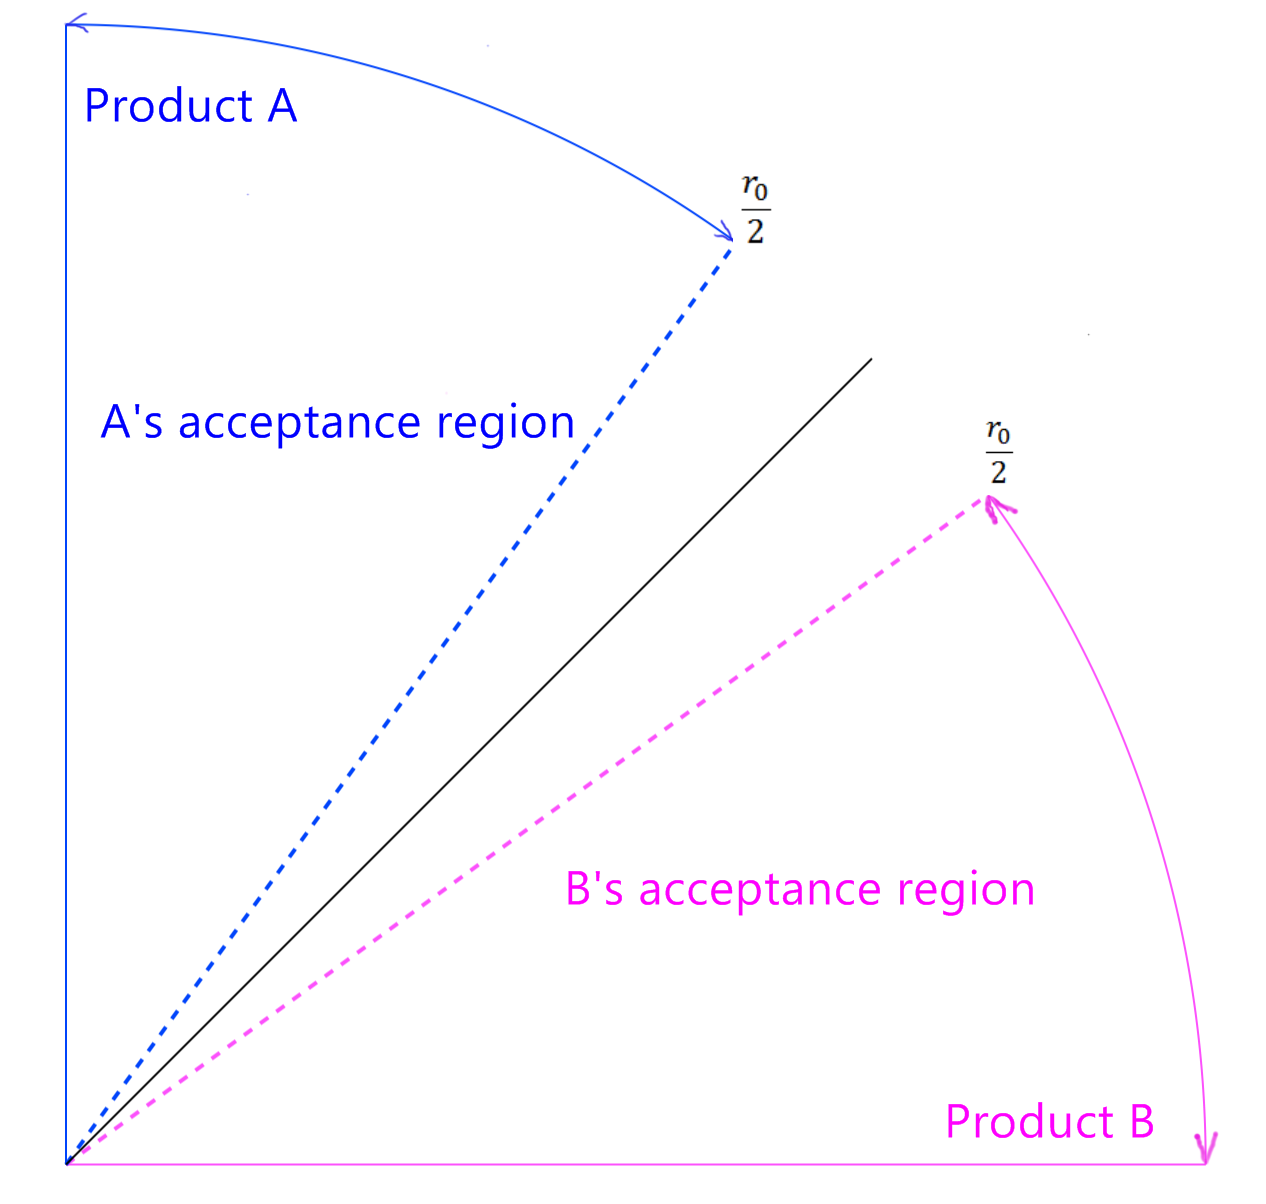
\includegraphics[width = 0.45\textwidth,height = 0.3\textheight]{lowlevel.png}
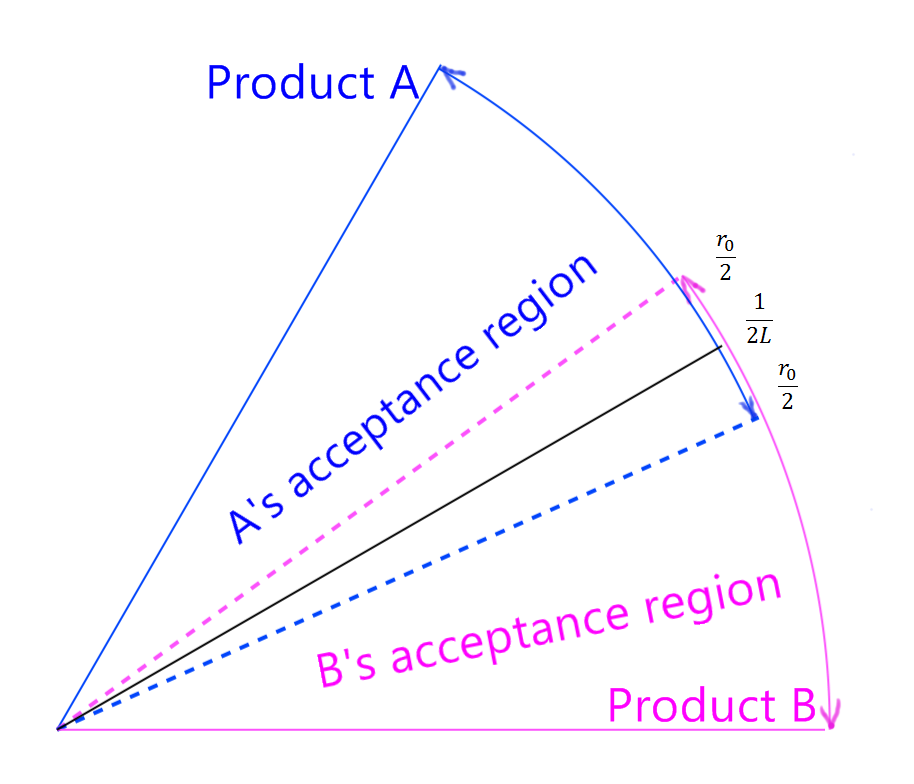
\includegraphics[width = 0.54\textwidth,height = 0.3\textheight]{highlevel.png}
\caption{Region of acceptance of Recommendation between two neighboring products}
\label{fig:twolevelROA}
\end{figure}
Figure \ref{fig:twolevelROA} (left)
is showing an example when $L = 4, r_0 = 0.2$. It plotted the region of consumers who accepted recommendations of a pair of neighboring products.

\subsection{high level of personalization, $L > \frac{1}{r_0}$}
When $L <\frac{1}{r_0}$, we have $\frac{r_0}{2} <\frac{1}{2L}$, the firm couldn't set the recommended product at the optimal price because of cannibalization. From some derivations, we get the best prices for each recommended product: the price is set such that $r^* = \frac{1}{2L}$. In this case, all consumers in the market will accept the recommendations rather than searching themselves.

Figure \ref{fig:twolevelROA}(right) plots the region of acceptance for consumers between two recommended products, when $L = 6, r_0 = 0.2$.
\subsection{Welfare results with different L: low lovel and high level}
Table \ref{tab:comp3welfare} summarizes how three welfare measures change with increasing level of personalization. 
\begin{table}[h]
\begin{tabular}[h]{|c|c|c|c|}
\hline 
L &  $\Delta$ Profit  & $\Delta$ CS & $\Delta$ Total Welfare \\
\hline \hline
L=0: No RS & 0 & 0&0\\
\hline
$0<L\leq \frac{1}{r_0} $: Low L & $\frac{1}{2} tr_0^2L$ & $\frac{1}{4}tr_0^2L$&$\frac{3}{4}tr_0^2L$\\
\hline
$L \geq \frac{1}{r_0}$: high L & $t(r_0 -\frac{1}{2L})$ & $\frac{t}{4L}$&$t(r_0 - \frac{1}{4L})$ \\
\hline
$L\to +\infty$: perfect personalization&$tr_0=s$&0&$tr_0=s$\\
\hline
\end{tabular}
\caption{Summary of welfare result: how increase in profit, cs and total welfare changes with the level of personalization L}
\label{tab:comp3welfare}
\end{table}
We saw a non-monotonic trend of the consumer surplus. The consumer surplus increases in L when L is below $\frac{1}{r_0}$, because when recommended products are fewer, by adding one product, more consumers will accept the recommendation, and there will be a same amount of increase in consumers surplus. When there are more differentiated recommended products, recommending another product will not attract more consumers, but increases the current prices of the recommended products and therefore decreases consumer surplus. 

The highest consumer surplus is obtained when $L = \frac{1}{r_0}$.

In constrast, profit and total welfare monotonically increase when the level of personalization L increases. Specifically, when $L \leq \frac{1}{r_0}$, profit and totalwelfare increases in L linearly, and beyond $\frac{1}{r_0}$,the two measures converge to $tr_0 = s$ with rate -1/L. 

The comparison of the trend of three welfare measures are shown in figure \ref{comp3welfare}.

\begin{figure}
\centering
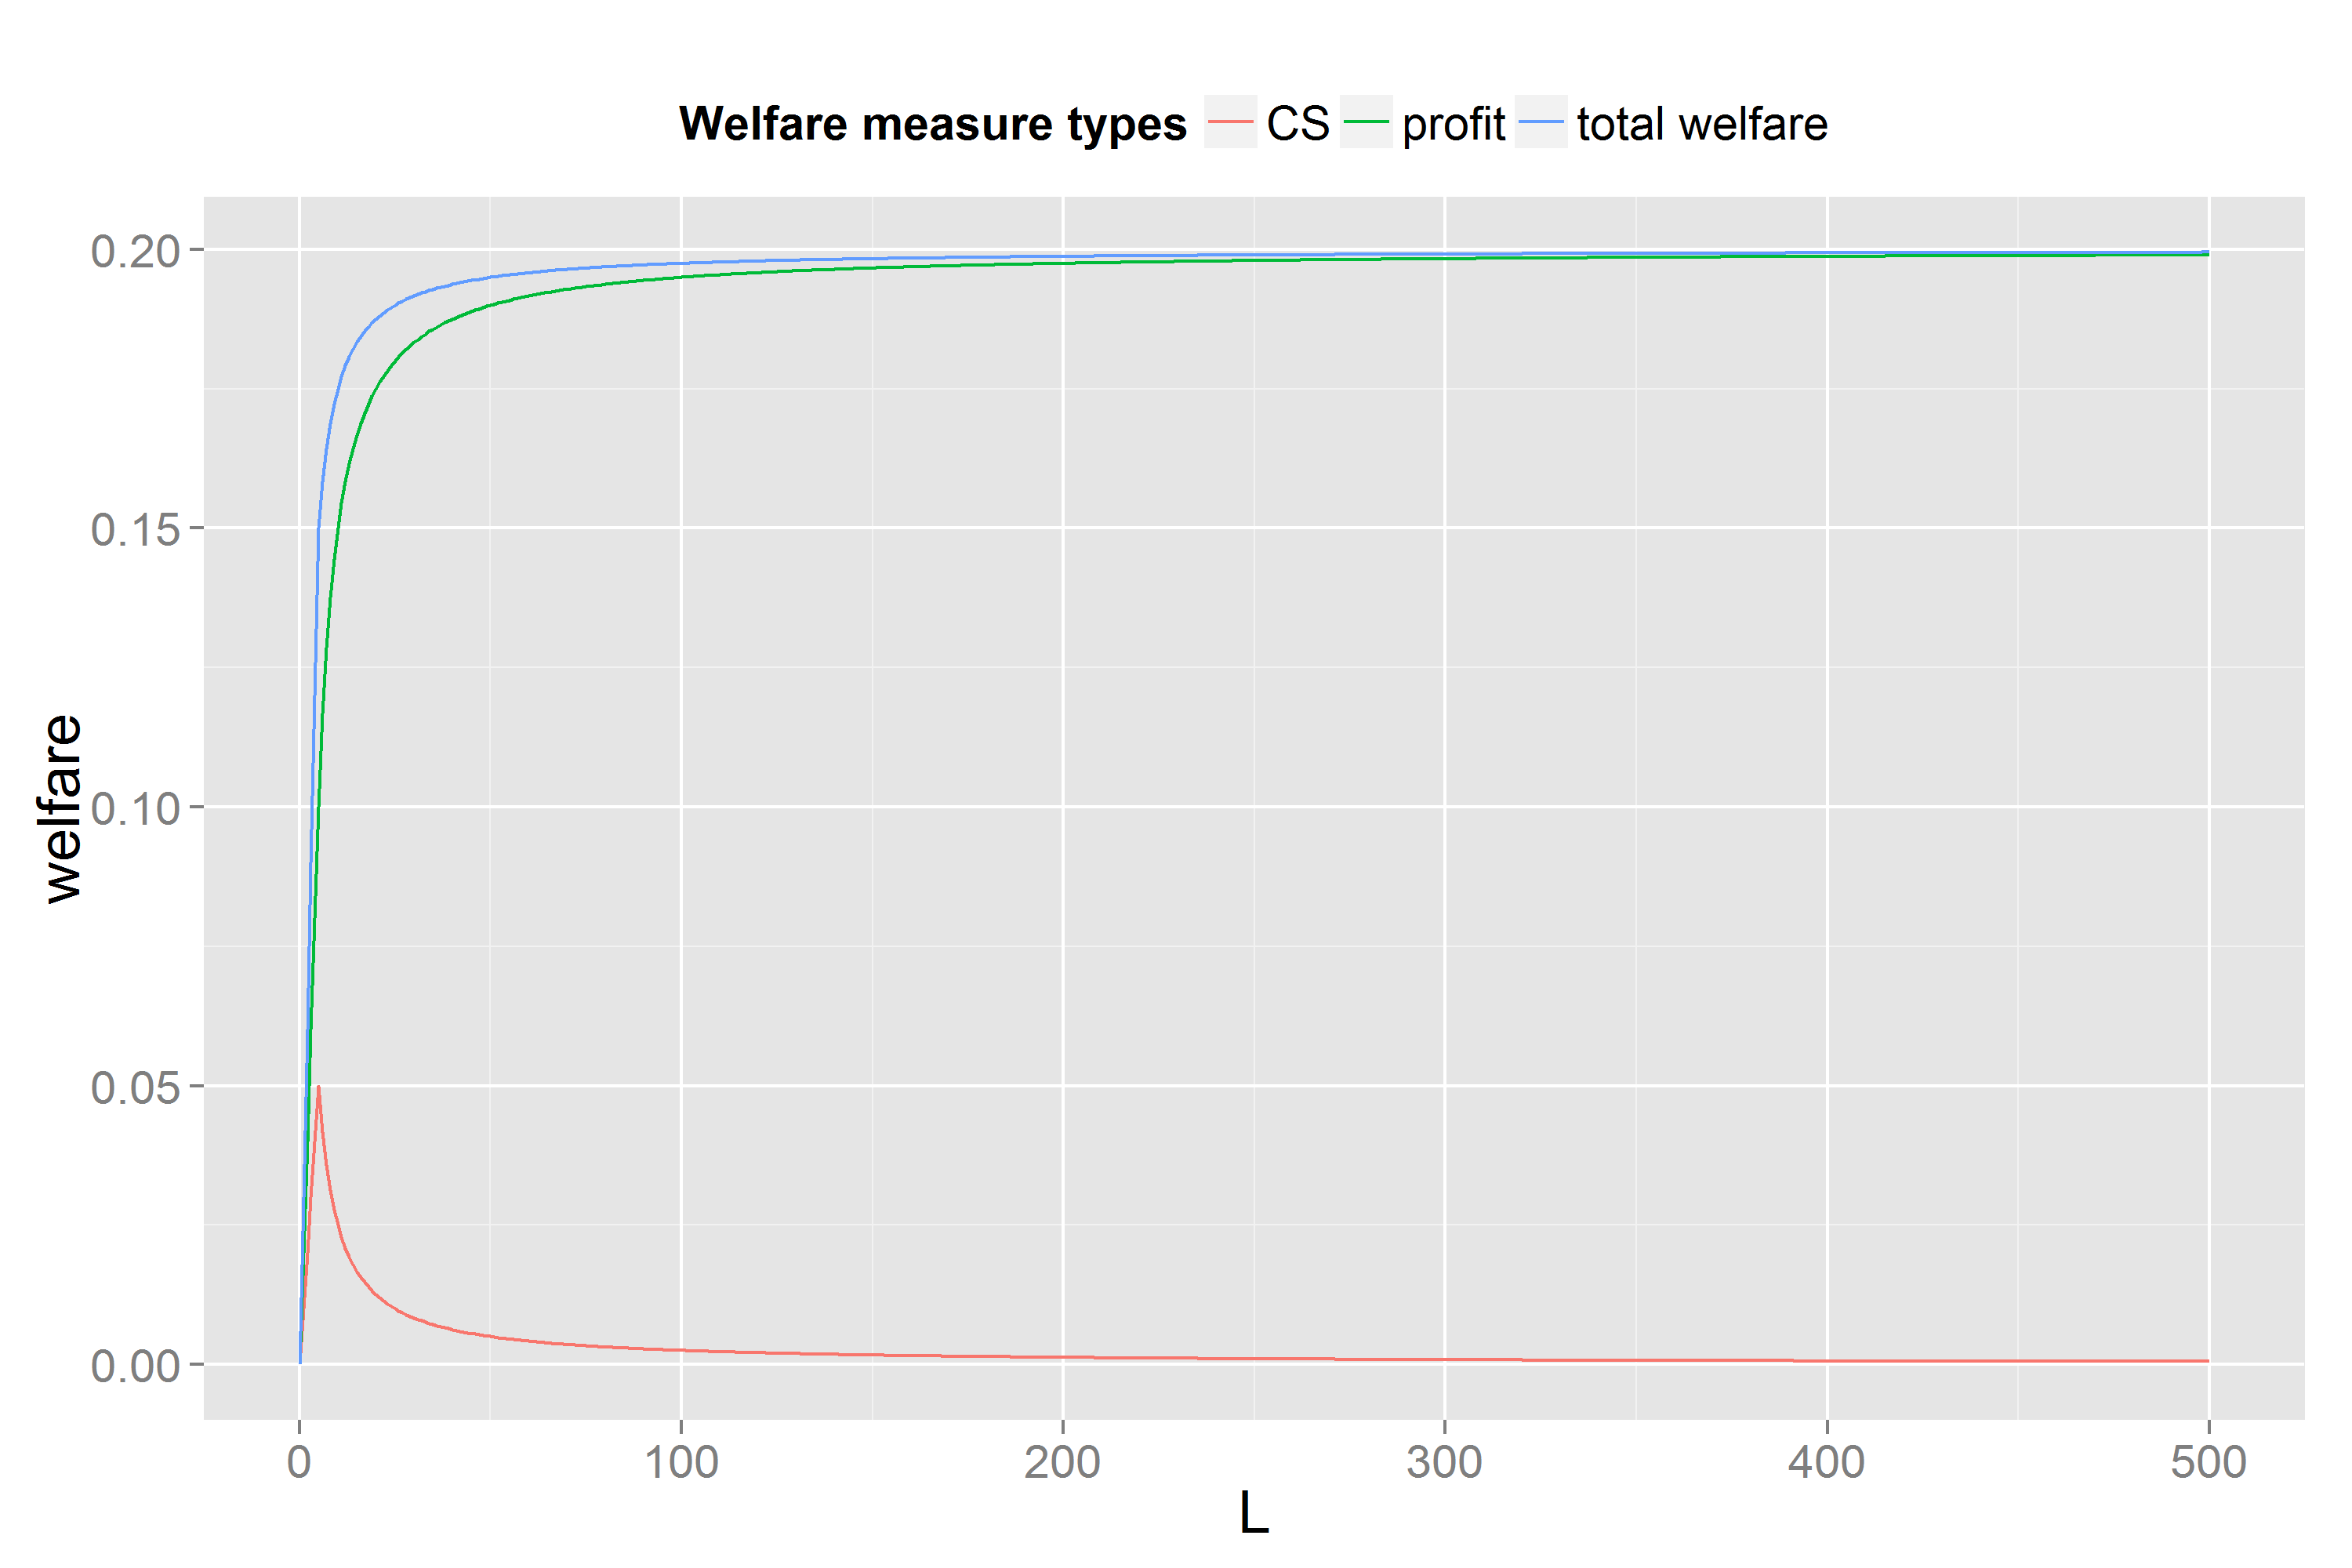
\includegraphics[width = 0.8\textwidth,height=0.5\textwidth]{compare3welfare.png}
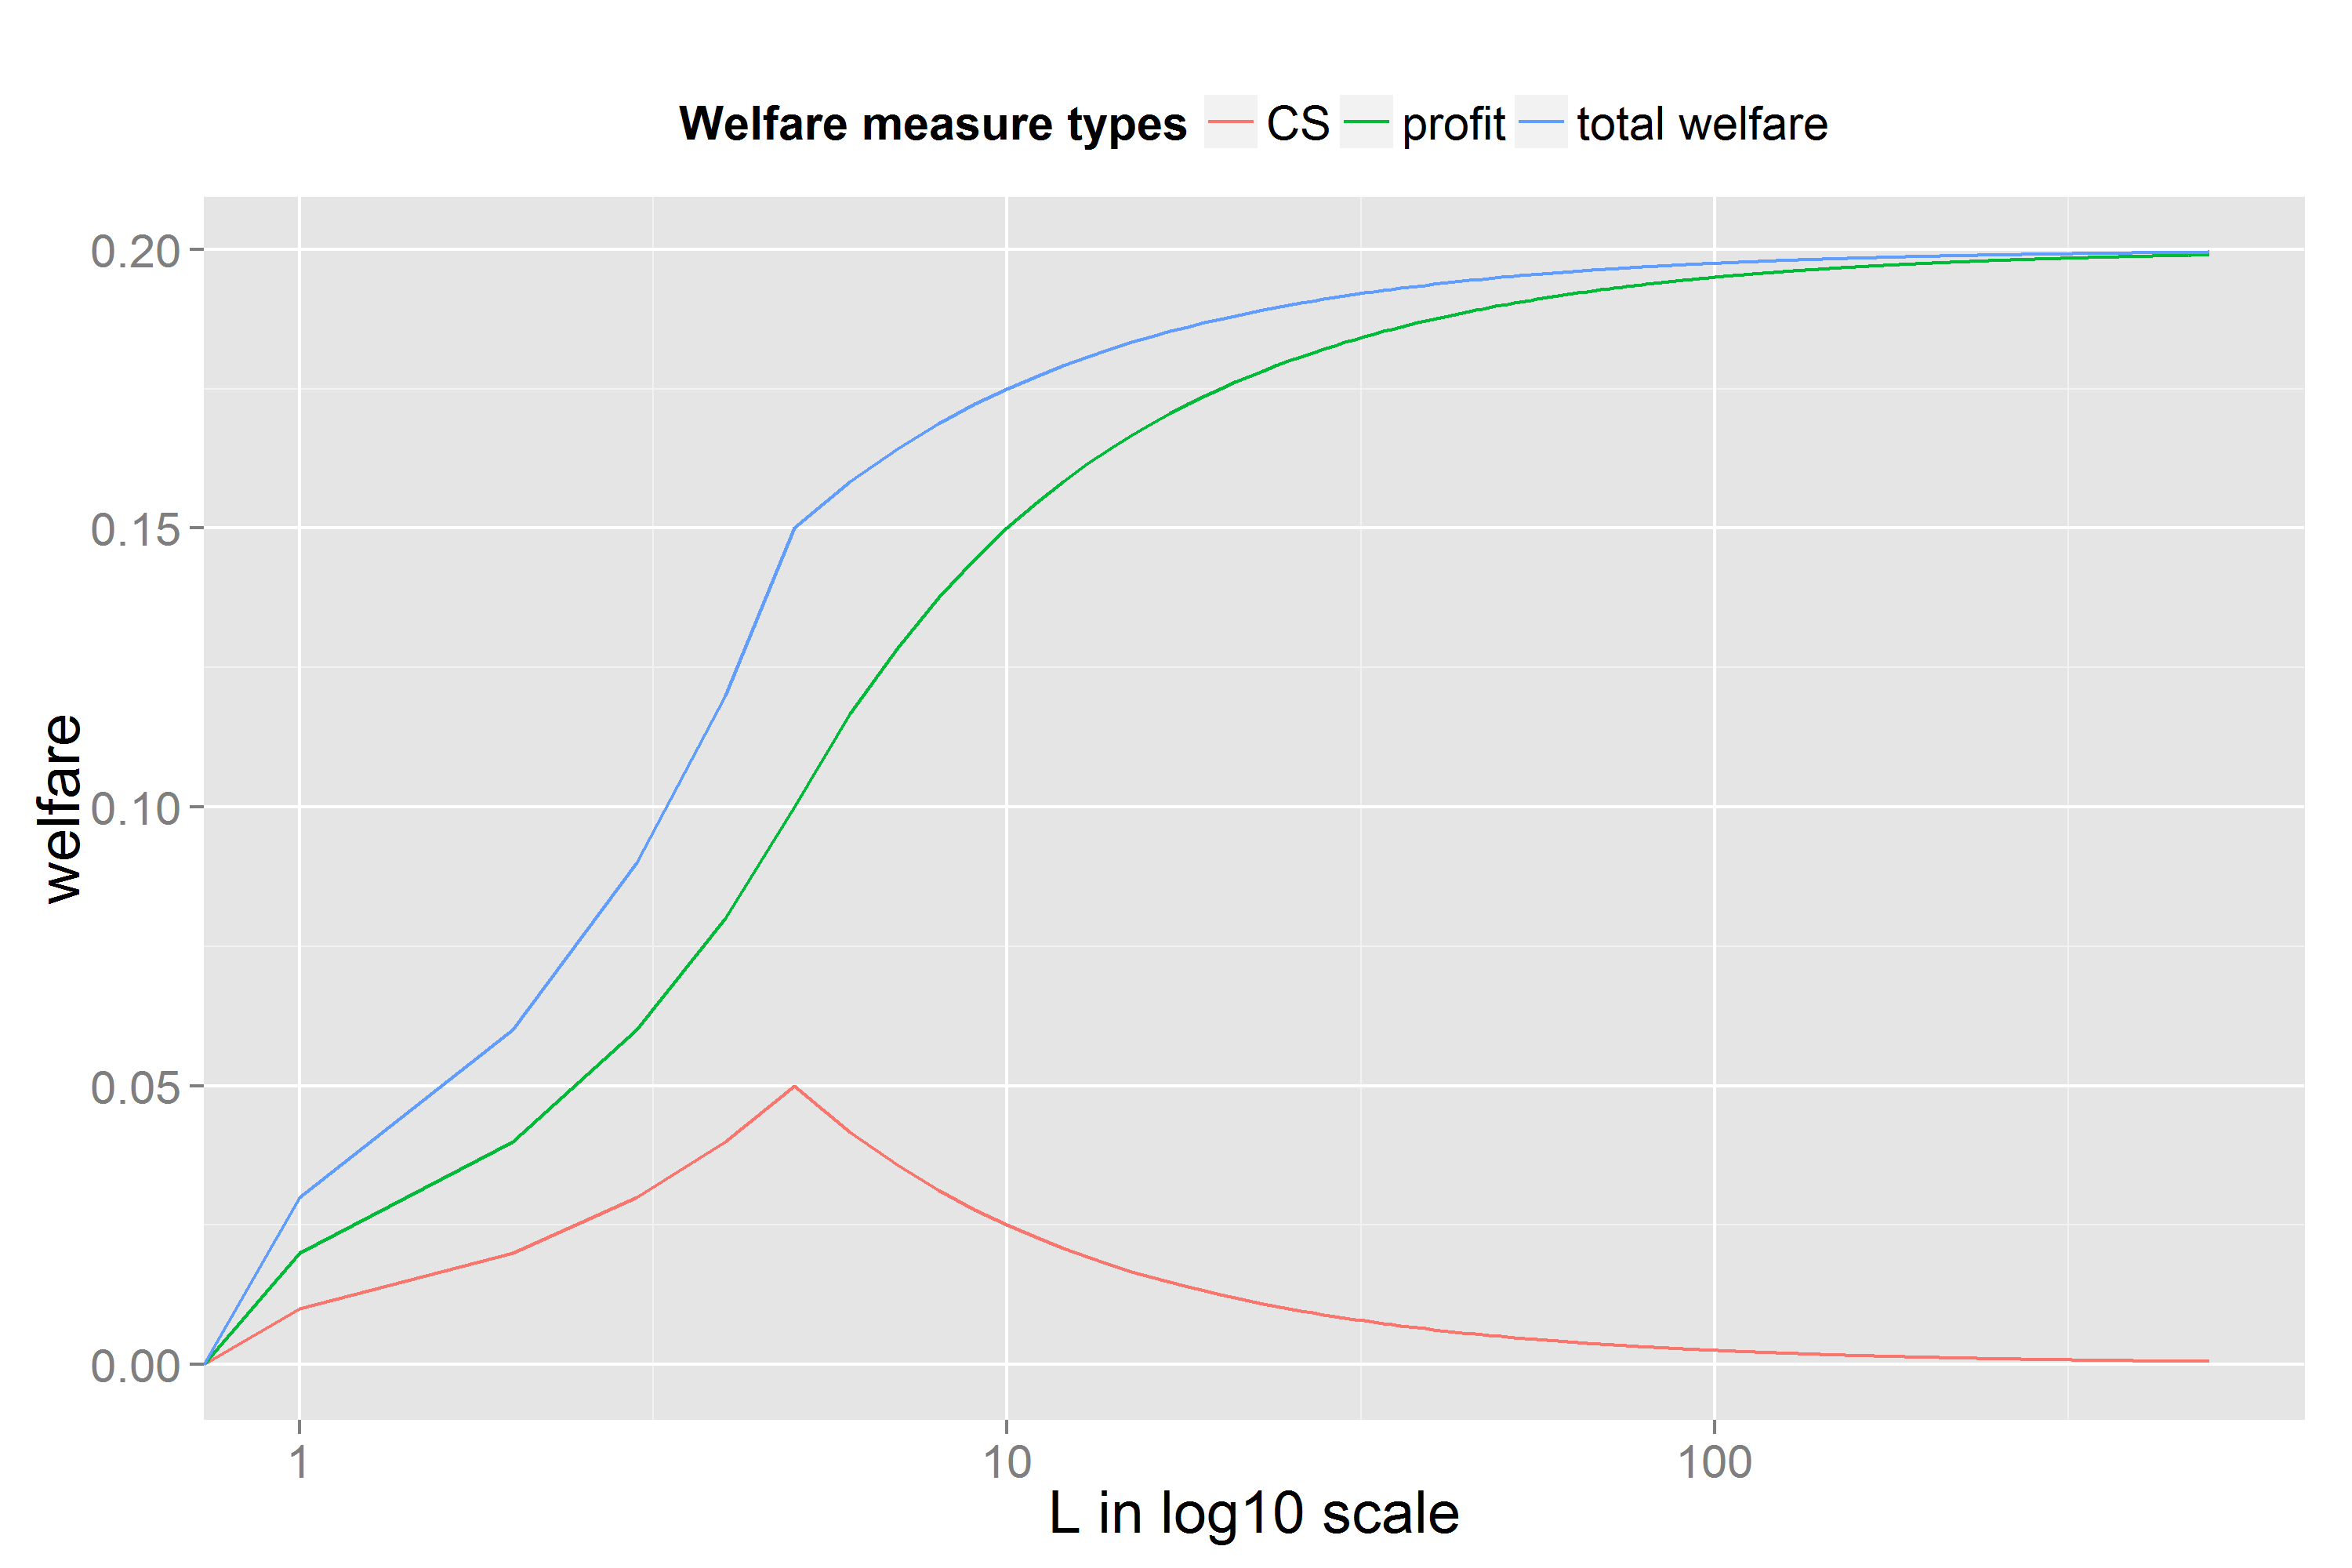
\includegraphics[width = 0.8\textwidth,height=0.5\textwidth]{compare3welfare-logscale.png}
\caption{Comparing how three welfare measures change in L ($r_0 = 0.2, t = 1$)}
\label{comp3welfare}
\end{figure}
\section{Price Discrimination}
We are interested in whether personalization and price discrimination are comparable in terms of how firm extracts surplus from consumers. From section 1 to section 4, we are talking about cases when price discrimination is not allowed. In this section, we want to explore the dynamics of price discrimination in this RS, and compare the welfare with previous result from personalized RS.

Without personalization, the firm will recommend only one product to consumers. Since the product circle is symmetric it makes no difference where the recommended product is located on the circle.

In order to make more profit than the catalog, the firm will target those consumers who are willing to accept the recommendation at a price higher than the catalog price $p_0$. To maximize this part of profit, the firm will show each consumer (at location $r$ distance away from the product) a personalized price (denoted by $p_r$) that makes him just be willing to accept the recommended product. 

\begin{align} p_l &= p_0 + t(r_0 - r )\\
s.t. {~}p_l &\geq p_0 \nonumber \\
 r& \leq r_0 \nonumber
\end{align}

The corresponding welfare changes are:
\begin{align}
\Delta \pi &= 2\int^{r_0}_0\nonumber (p_r-p_0) dr\\
&=2\int^{r_0}_0[t(r_0-r)]dr \nonumber \\
&=tr_0^2\\ 
\Delta CS &=2\int_0^{r_0} [V-p_r-tr - (V-p_0-s)] \nonumber\\
&=2\int^{r_0}_0(0)dr = 0\\
\Delta TW &=\Delta \pi + \Delta CS = tr_0^2 \nonumber \\ 
\end{align}

The above derivations are based on assumption that $r_0 \leq 1$. Under this assumption, $tr_0^2 < tr_0 = s$. The price-discriminated-only RS ($\Delta TW = tr_0^2$) generate less total welfare than the perfect personalized RS ($\Delta TW = tr_0 = s$). The cause of this phenomenon is that perfect-personalized-only RS saves all consumers search costs, and in contrast, the price-discriminated-only RS saves some consumers search costs while at the mean time creating misfit costs for them.

Either price-discriminated-only RS and perfect-personalized-only RS give zero consumer surplus.

If we combine price discrimination with personalization, the result is shown in the following table \ref{tab:combine}:
\begin{table}[ht]
\begin{tabular}[h]{|c|c|c|c|}
\hline 
L2 &  $\Delta$ Profit  & $\Delta$ CS & $\Delta$ Total Welfare \\
\hline \hline
L2=1: No personalization & $tr_0^2$ & 0&$tr_0^2$\\
\hline
$0<L2\leq \frac{1}{2r_0} $: Low L2 & $ tr_0^2L$ & 0&$ tr_0^2L$\\
\hline
$L2 \geq \frac{1}{2r_0}$: high L2 & $t(r_0 -\frac{1}{4L})$ & 0&$t(r_0 - \frac{1}{4L})$ \\
\hline
$L2\to +\infty$: perfect personalization&$tr_0=s$&0&$tr_0=s$\\
\hline
\end{tabular}
\caption{Summary of welfare result when combing personalization and price discrimination}
\label{tab:combine}
\end{table}
The result shown in table \ref{tab:combine} is consistent with our previous result without modeling search cost:When the personalization level L is finite, the effect of price discrimination is to redistribute welfare between firm and consumers. When there is perfect personalization, i.e. each consumer is recommended a different personalized product, then consumer surplus will go to zeros with or without price discrimination.

Figure \ref{fig:tw-comp} and figure \ref{fig:pi-cs-comp} plotted the trend of welfare change in L comparing with vs. without price discrimination.

\begin{figure}
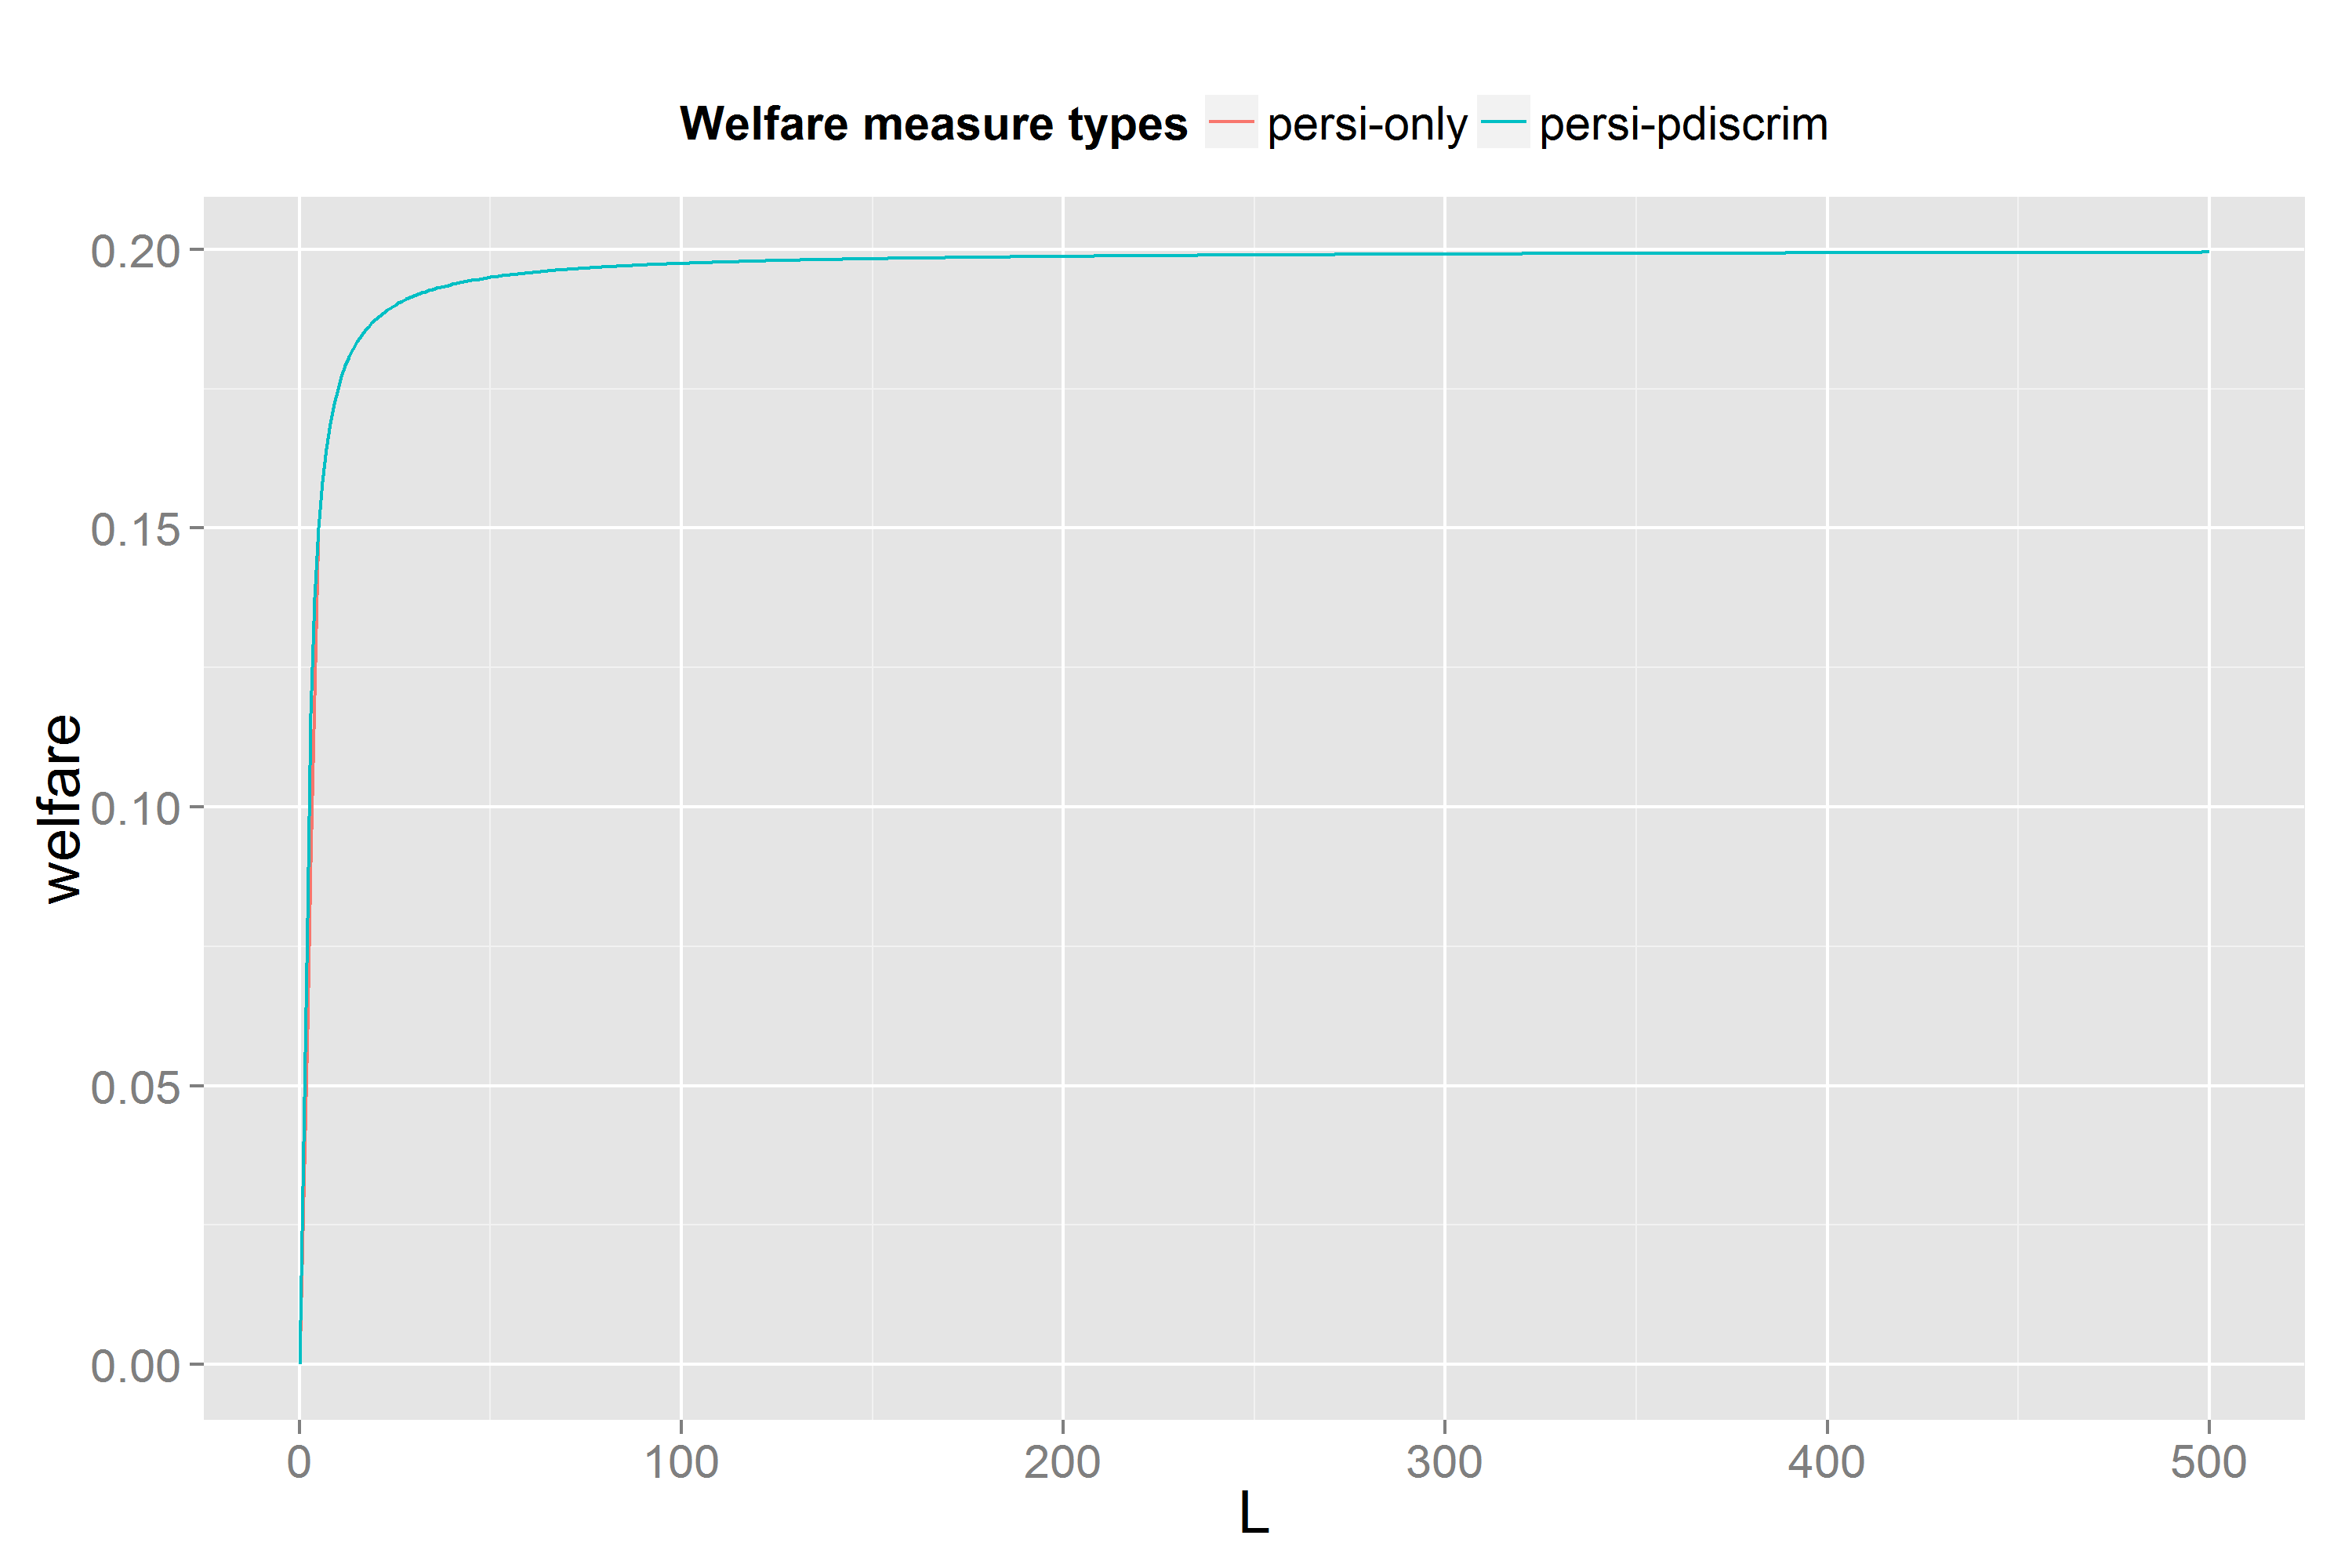
\includegraphics[width= 0.5\textwidth ,height =0.3\textheight]{compareTW-persi-pdiscrimvspersi-only.png}
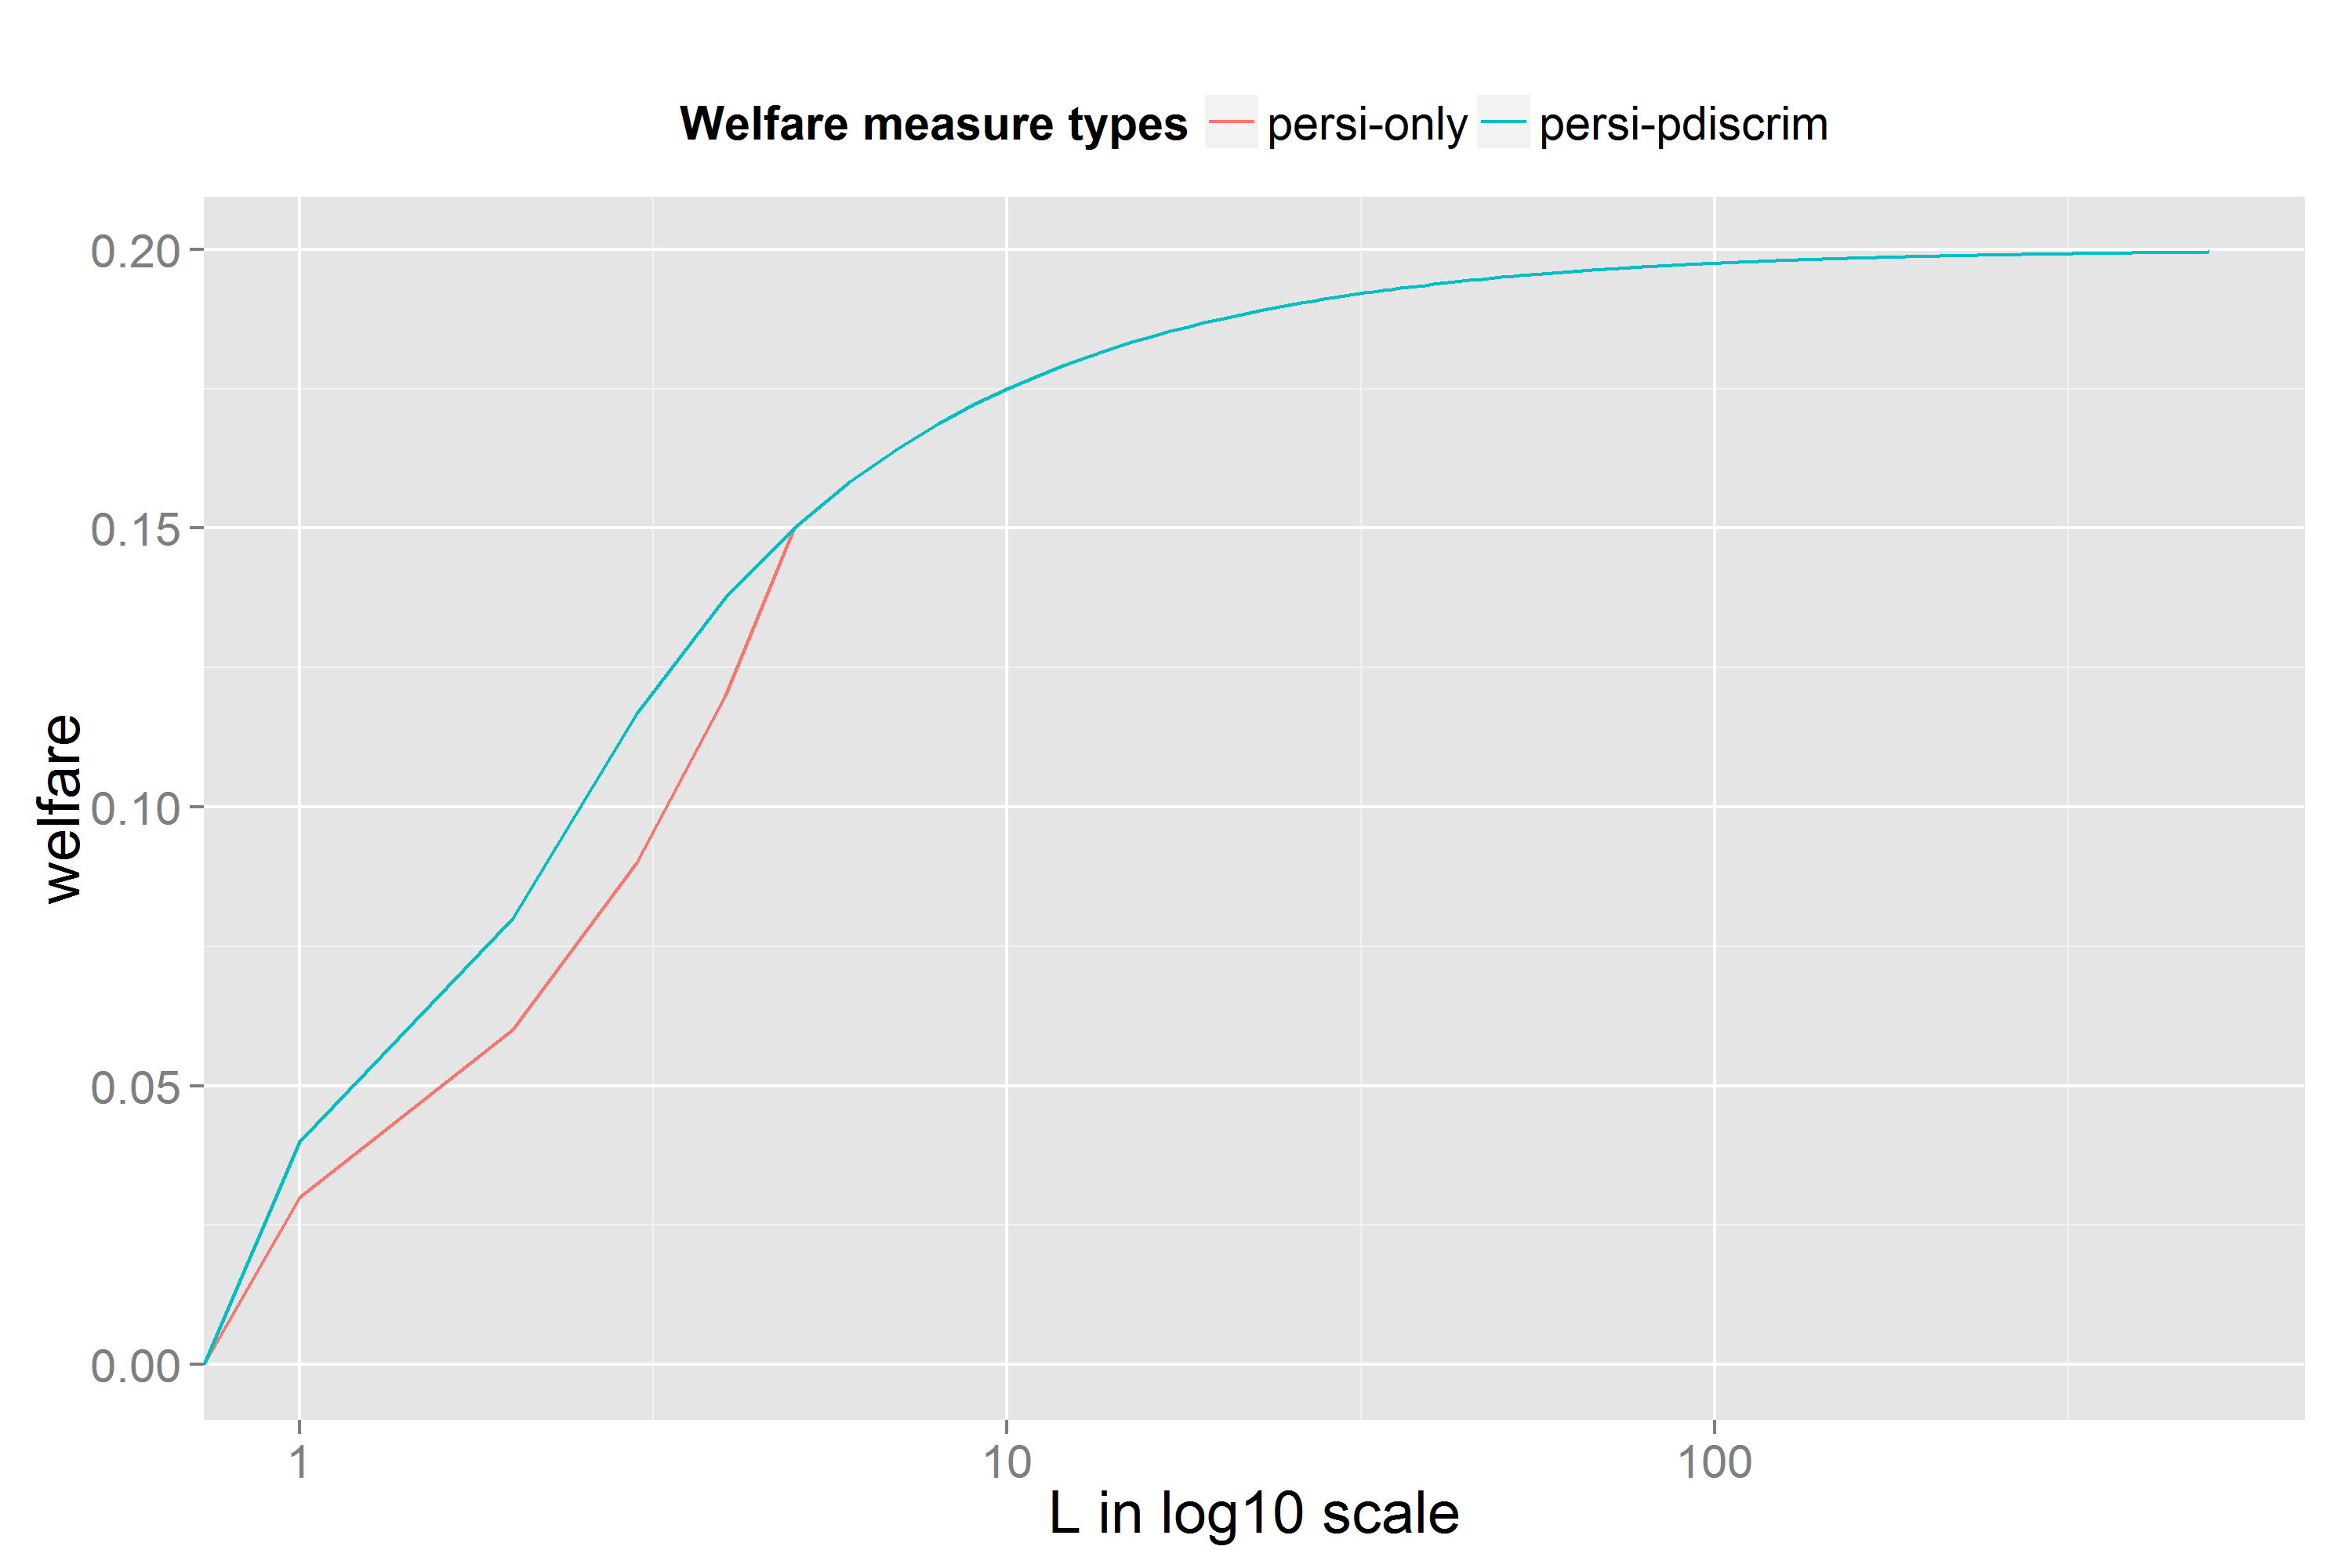
\includegraphics[width= 0.5\textwidth ,height =0.3\textheight]{compareTW-persi-pdiscrimvspersi-only-logscale.png}
\caption{Total welfare with(green) or without(red)price discrimination}
\label{fig:tw-comp}
\end{figure}

\begin{figure}
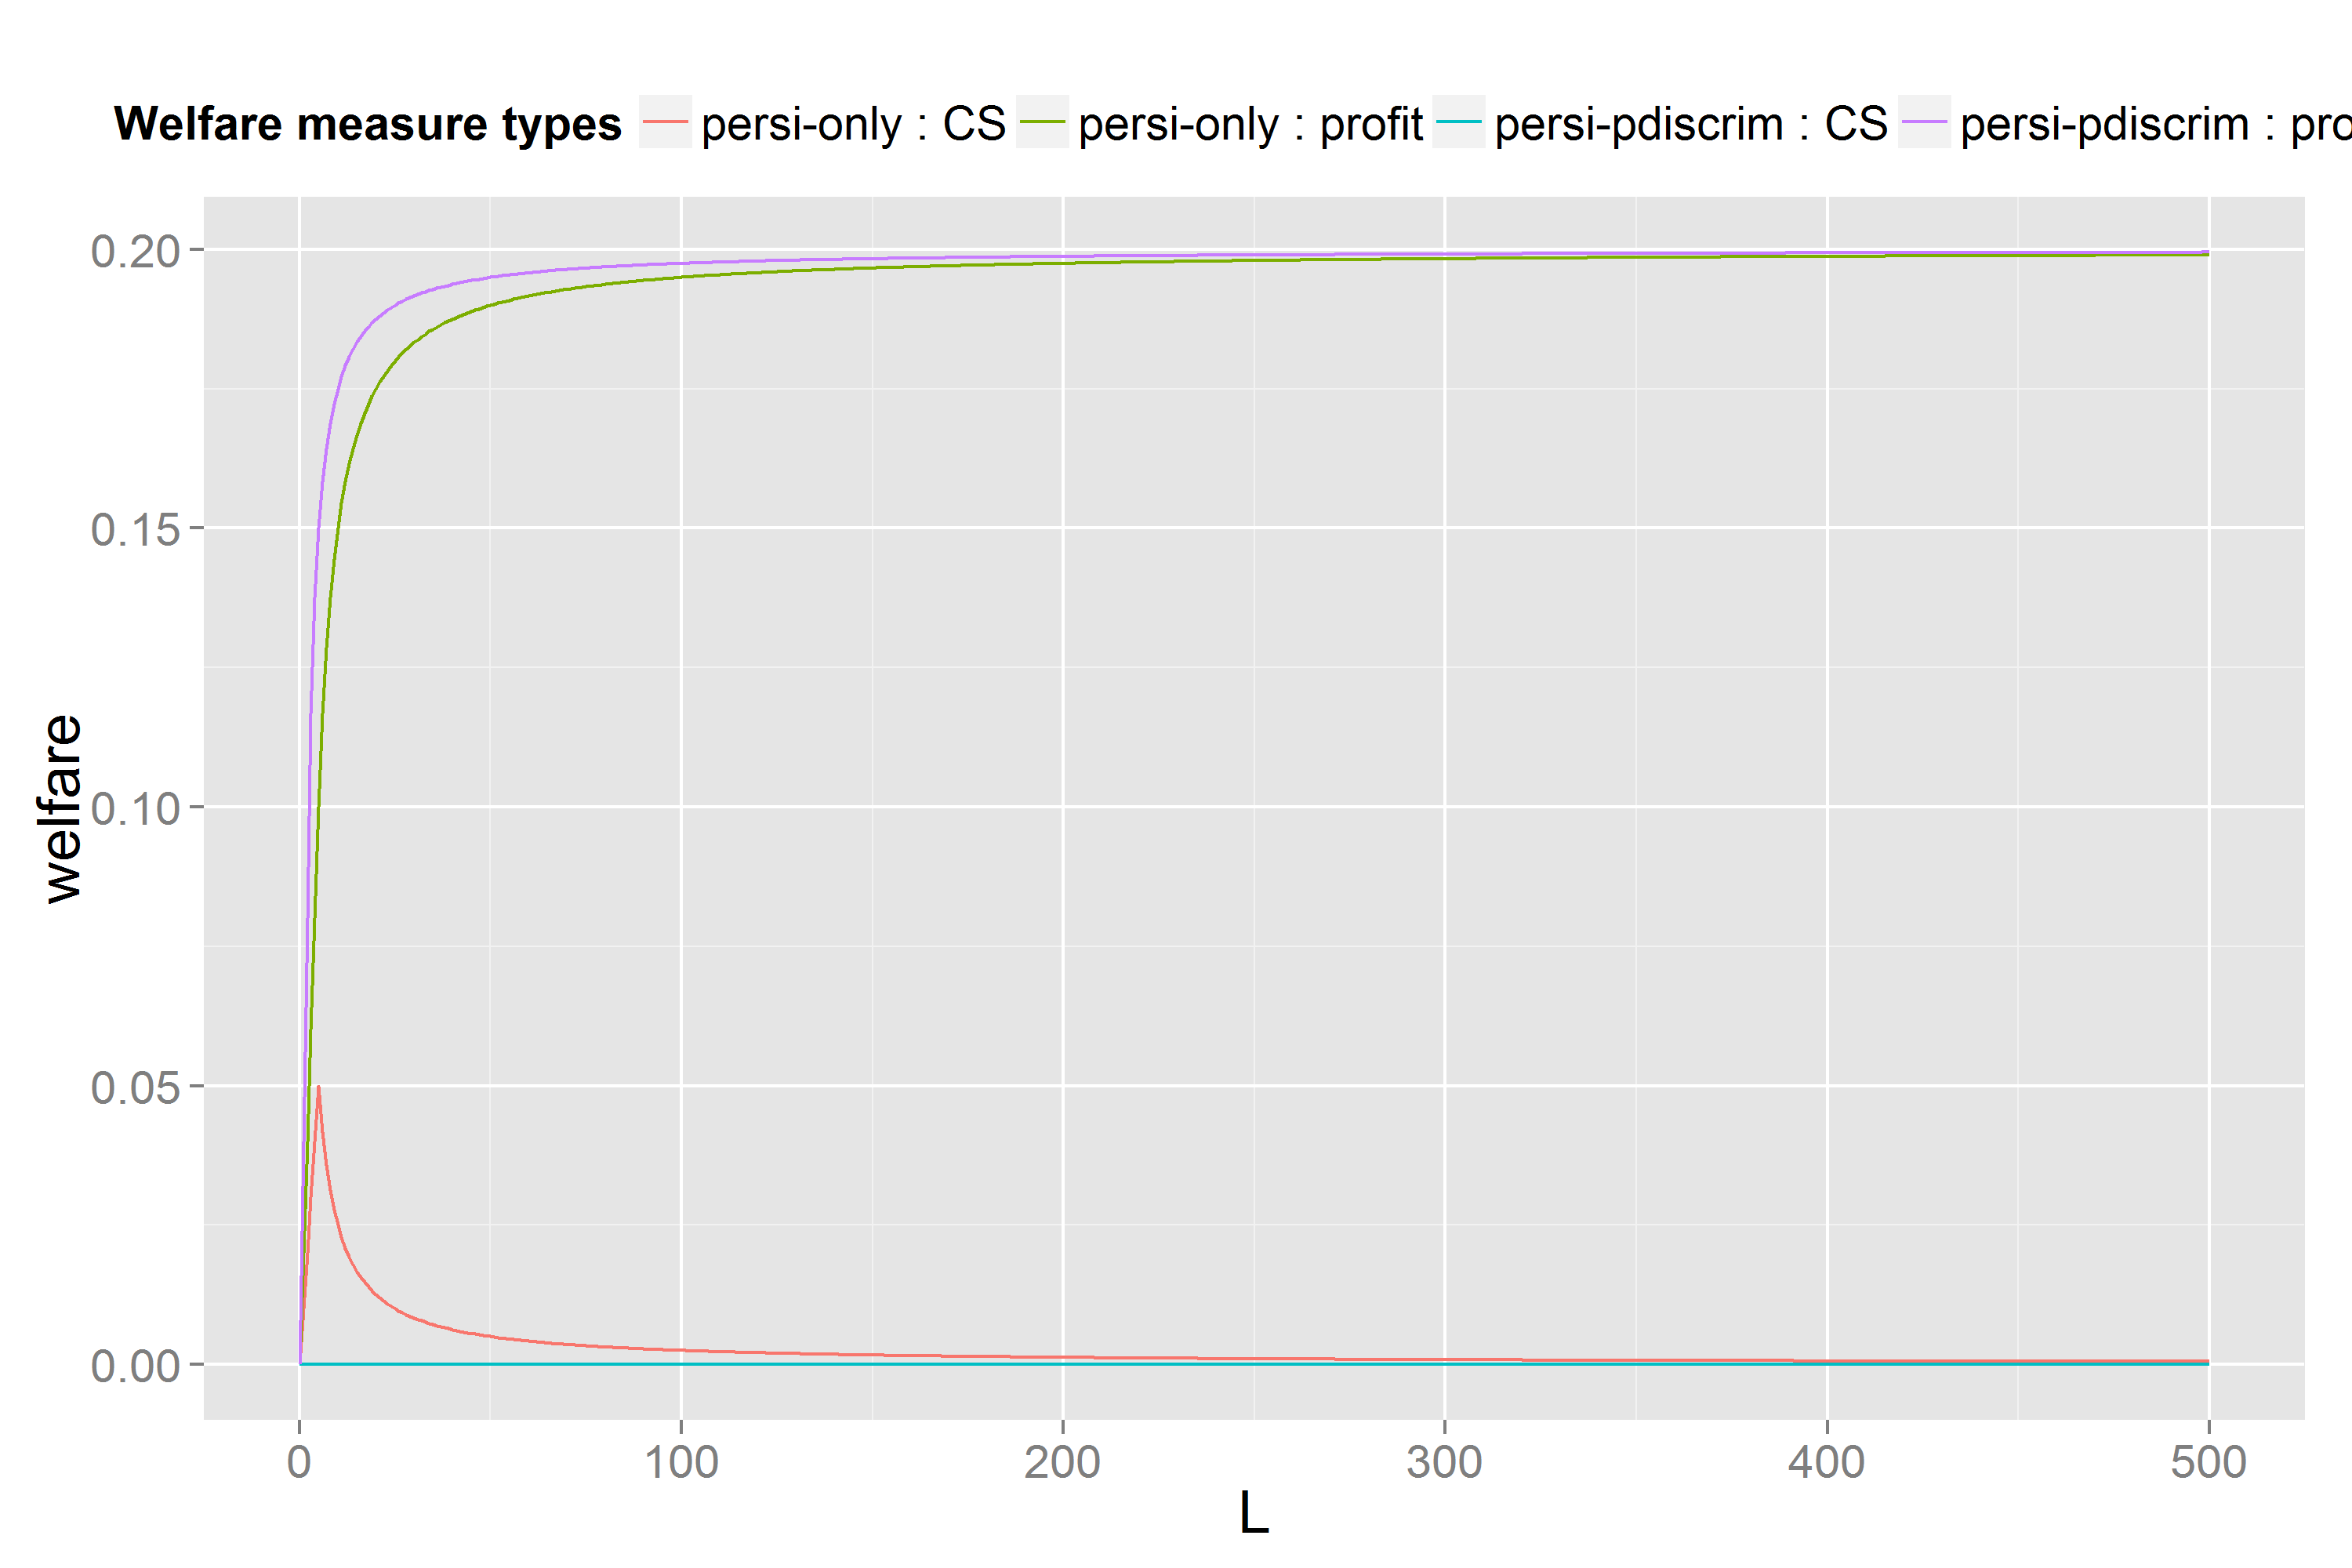
\includegraphics[width= 1\textwidth ,height =0.6\textheight]{compareTprofitANDCS-persi-pdiscrimvspersi-only.png}
\caption{Total welfare with(blue for cs,purple for profit) or without(red for cs, light green for profit) price discrimination}
\label{fig:pi-cs-comp}
\end{figure}
\end{document}  